\chapter{Introduction}
There are fundamental limitations to what can be done with serial/non-parallel computing. If you want to process a great deal of data simultaneously, a serial computer will only be able to handle a subset of the data at any given point.

A parallel computing system combines multiple computers/computing units so that they can be used to work on the same problem simultaneously. If a problem is "parallelisable", then it can be split up and executed across multiple machines.

\section{Architectures}
There are two types of computer architectures that are built on top of interconnected multiple processors:
\begin{itemize}
\item \textbf{Tightly coupled systems} have a single system-wide memory space shared by all the processors (that is, memory addresses for one processor are valid in another processor). \begin{figure}[h]
\centering
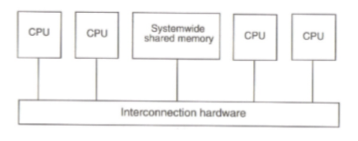
\includegraphics[width=0.5\linewidth]{figures/screenshot001}
\caption{Tightly coupled system}

\label{fig:screenshot001}
\end{figure}
\item \textbf{Loosely coupled systems} do not share memory; each unit in the system has its own memory store that no other unit can access. \begin{figure}
\centering
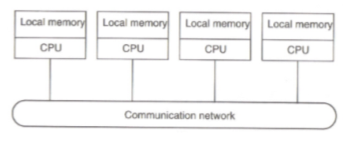
\includegraphics[width=0.7\linewidth]{figures/screenshot002}
\caption{Loosely coupled system}
\label{fig:screenshot002}
\end{figure}

\end{itemize}

\section{Distributed Systems}
The textbook definition of a distributed system:
\begin{quote}
A distributed system is a collection of independent computers that appears to its users as a single coherent system.
\end{quote}

In this definition, it is important that each computer is \textbf{independent} - that is, they can operate individually - and that the entire system appears as a \textbf{single coherent system} - users are not necessarily aware that the system is composed of multiple computing units.

Additionally, it is worth noting that components that are located on separate networked computers (e.g. Process A running on Computer 1, Process B running on Computer 2) communicate using message passing only - that is, they do not share memory.

The rise of distributed systems has been attributed to a variety of causes, including the prevalence of powerful microprocessors (especially conventional consumer processors, such as the Intel x86 line) and the availability of high-speed computer networking technology.

\subsection{Models}
A distributed computing system can be structured in a variety of different ways. These can be roughly categorised into one of the following five models.

\subsubsection{Minicomputer}
The minicomputer model is an extension of the centralised time-sharing systems of the 1970s. There are several minicomputers connected by a communication network, with each minicomputer having several users logged in simultaneously.

\begin{figure}[h]
\centering
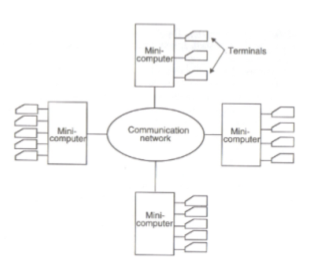
\includegraphics[width=0.5\linewidth]{figures/screenshot003}
\caption{Minicomputer model}
\label{fig:screenshot003}
\end{figure}

This model is useful when resources must be shared with remote users, and was used for early ARPAnet (the military/university precursor to the Internet).

\subsubsection{Workstation}
The workstation model uses multiple workstations that communicate to each other using a communication network. These workstations often have spare computing power available, which is leveraged by the system as part of its operation.

Essentially, a user uses their workstation to submit a job to be run. These jobs are then distributed across the workstations on the network, allowing for work to be distributed and a more efficient allocation of resources than letting workstations idle.

\begin{figure}[h]
\centering
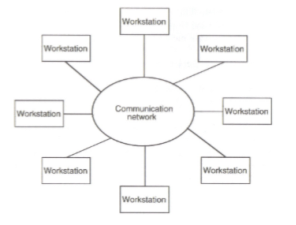
\includegraphics[width=0.5\linewidth]{figures/screenshot004}
\caption{Workstation model}
\label{fig:screenshot004}
\end{figure}

However, there are several issues that must be resolved for efficient use of this model. These include:
\begin{itemize}
\item finding an idle workstation: the network must be able to allocate a workstation for execution of the job. If there is no such workstation available, the execution of the job may be delayed.
\item transferring the job: when a workstation is available, the job can be transferred to it; but the actual method of transfer may be complicated, as the state of the job (i.e. the work completed to date) will also need to be transferred.
\item control of a remote process: the system must be able to efficiently allocate and control processes on other workstations from the current workstation, which may result in complications
\end{itemize}

This model has been used for the Sprite system, as well as in Xerox PARC.

\subsubsection{Workstation-server}
\begin{figure}
\centering
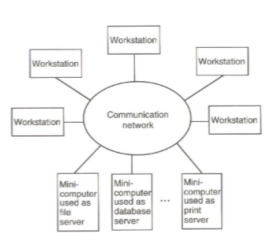
\includegraphics[width=0.5\linewidth]{figures/screenshot005}
\caption{Workstation-server model}
\label{fig:screenshot005}
\end{figure}

The workstation-server model is a variant on the workstation model that adds several minicomputers to the system. These minicomputers provide services that all workstations may need at any given moment (and thus cannot be treated as a temporary job as would be the case with the workstation model). These services include file servers, database servers, and more.

There does not need to be a one-to-one allocation between a service and a minicomputer server; for example, multiple servers can provide a single service. This increases redundancy, which in turn increases reliability and provides better scalability.

An example of this model is the V-System.

\subsubsection{Processor-pool}
\begin{figure}[h]
\centering
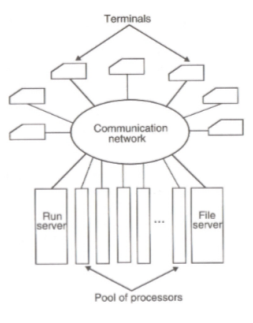
\includegraphics[width=0.5\linewidth]{figures/screenshot006}
\caption{Processor-pool model}
\label{fig:screenshot006}
\end{figure}

The processor-pool model is based around the observation that a user may have extremely varying computing demands, ranging from no computing power to a significant amount for a short period of time.

Given this, users are given terminals that have no independent computing power of their own. These terminals connect to the processor-pool, which is managed by a \textit{run server}. This run server allocates processors to users as required, allowing for efficient utilisation of the servers.

Users do not have a home machine; instead, they log onto the entire system and are allocated processing power as required.

Examples include Amoeba, Plan 9, and Cambridge DCS.

\subsubsection{Hybrid}
The hybrid model combines the workstation-server and processor-pool models with the aim of maximising the advantages of both. It augments the workstation-server model with a pool of processors.

This means that in a hybrid system, there are powerful workstations, servers and a pool of processors. These workstations can access resources on the servers, conduct work amongst themselves, or schedule high-load work on the processor pool.

As this requires the most resources out of all the models discussed, it is also the most expensive to implement.

\subsection{Distribution Model}
There are several models for how resources are distributed and/or made visible to nodes of a distributed system. Some of these include:

\begin{itemize}
\item \textbf{File Model}: resources are modelled as files on the file system, and are accessible through regular file APIs.
\item \textbf{Remote Procedure Call Model}: resources are modelled as function calls, and can be accessed by calling the functions and retrieving their results.
\item \textbf{Distributed Object Model}: resources are modelled as objects (a combination of data and functions relating to the data), and can be accessed by accessing the representation of the object.
\end{itemize}

\subsection{Advantages}
\begin{itemize}
\item \textbf{Economics}: Microprocessors provide a better performance/price ratio than mainframes.
\item \textbf{Speed}: A distributed system can offer more computing power than a mainframe, especially as the number of the nodes in the system go up. A concrete example of this is splitting a database into many small databases, which can reduce the average response time by increasing the ratio of database servers to clients.\begin{figure}[h]
\centering
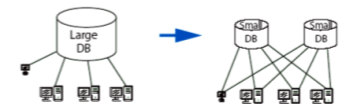
\includegraphics[width=0.5\linewidth]{figures/screenshot008}
\caption{Single DB server vs multiple DB servers}
\label{fig:screenshot008}
\end{figure}
\item \textbf{Reliability}: The system can operate in a degraded state when it is partially unavailable; that is, a perfectly-redundant system with 5\% of the system down would only experience 5\% performance degradation.
\item \textbf{Incremental growth}: The system can be incrementally grown by adding new nodes.
\item \textbf{Sharing}: Many users can be granted access to common resources, such as a database and peripherals.
\item \textbf{Communication}: Humans using the system can communicate to each other using the abstraction offered by the system.
\item \textbf{Effective Resource Utilisation}: A distributed system can distribute any given workload over available machines in the most cost effective and efficient way possible.
\end{itemize}

\subsection{Disadvantages}
\begin{itemize}
\item \textbf{Software}: Distributed software is harder to develop than centralised software.
\item \textbf{Networking}: The networking link cannot be assumed perfect; it may saturate (i.e. the network is completely used and cannot accept new connections) or experience other issues.
\item \textbf{Security}: Data distributed across multiple nodes cannot be assumed to be secure, as the "easy access" nature of distributed data also applies to secure data.
\end{itemize}


\subsection{Challenges}
\subsubsection{Heterogenity}
A distributed system can feature variation in, but not limited to:
\begin{itemize}
	\item \textbf{Networks}: The same protocol may not be used to communicate between nodes. Even if it is, the performance may vary within the network (especially with regards to network topology).
	\item \textbf{Computing hardware}: Different processors represent data differently (little vs big-endian, as an example).
	\item \textbf{Operating systems}: Message exchange may work differently between operating systems.
	\item \textbf{Programming languages}: Programming languages represent characters and data structures differently from each other.
	\item \textbf{Implementations by different developers}: Developers must have a common specification or standard; otherwise, their implementations of the system may be unable to co-operate.
\end{itemize}

\subsubsection{Openness}
New nodes and services can be added to a distributed system, but existing nodes may not know how to interface or interact with these new nodes. To alleviate this, specifications and/or interfaces for the new components should be published ahead of time.

\subsubsection{Transparency}
\label{sssec:transparency}
A distributed system, as defined, conceals its distributed nature by masquerading as a single computer. An example of this might be the World Wide Web, which largely hides its distributed nature.

In the context of distributed systems, the term \textit{transparency} refers to hiding something \footnote{This is clearly wrong by any English dictionary - \textit{opaqueness} is the right term to use - but someone made a mistake a long time ago and we have to live with it now.}.

Classifications of transparency:

\begin{itemize}
\item \textbf{Access transparency}: Data and resources can be used in a consistent way.
\item \textbf{Location transparency}: A user cannot determine where resources are located.
\item \textbf{Migration transparency}: Resources can move without changing the identifier used to access them.
\item \textbf{Replication transparency}: A user cannot determine how many copies exist of a resource.
\item \textbf{Concurrency transparency}: Multiple users can share resources automatically.
\item \textbf{Failure transparency}: A user does not recognise resource failure.
\item \textbf{Performance transparency}: Systems are reconfigured to improve performance as loads vary.
\item \textbf{Scaling transparency}: Systems can expand in size without changing the structure of the system or the programs to run on the system.
\end{itemize}

\subsubsection{Performance}
An effective distributed system aims to produce high performance from a collection of cheap computers; this will be largely dependent on the workload and the distribution scheme.

There are two kinds of parallelism:

\begin{itemize}
\item \textbf{Fine-grained parallelism}: Small programs are executed in parallel. This results in a large number of messages; the communication overhead may result in a reduction in the performance gain from parallel processing.
\item \textbf{Coarse-grained parallelism}: Large, compute-intensive programs are executed in parallel. As these programs are mostly independent, the communication overhead is limited compared to fine-grained parallelism.
\end{itemize}

The maximum aggregate performance of the system can be quantified in terms of the maximum aggregate floating-point operations per second, as shown below:
\[ P = N \times C \times F \times R \]
where $P$ is the performance in FLOPS (floating point operations per second), $N$ is the number of nodes, $C$ is the number of CPUs, $F$ is the number of floating point operations per clock period, and $R$ is the clock rate of each CPU.

Similar values can be calculated for MIPS (million instructions per second).

\subsubsection{Scalability}
A distributed system should naturally scale with increasing numbers of nodes. However, the scaling algorithm may break down at increasingly large scales of thousands of nodes or more.

Challenges may arise from having centralised the following:

\begin{itemize}
\item \textbf{Centralised components}: A single server (e.g. a mail server) for all users.
\item \textbf{Centralised tables}: A central data store (e.g. a single online telephone book) for all nodes.
\item \textbf{Centralised algorithms}: Algorithms dependent on information available only from the complete system (e.g. routing based on complete information).
\end{itemize}

To mitigate these, the following techniques can be used:

\begin{itemize}
\item No node in the system is fully aware of the state of the system.
\item Nodes are only allowed to make decisions based on local state.
\item Algorithms should be designed in such a way to avoid their invalidation upon the failure of a single node.
\end{itemize}

Scalability can be quantified using the following formula:
\[ S = \frac{T_1}{T_N}  \]
where $T_1$ is the wall-clock time for a single processor, and $T_N$ is the wall-clock time over $N$ processors.

A scalability figure close to $N$ implies that the program scales well. This metric can be used to estimate the optimal number of processors for an application.

Additionally, the utilisation of the system can be calculated as such:
\[ U = \frac{S(N)}{N} \]
Ideally, $U$ would be close to $1$ (or $U \times 100\%$ would be close to $100\%$).

\subsubsection{Reliability}
Due to the large number of components in a distributed system, the probability of \textit{any} component failing is much higher than the probability of a non-distributed system failing. The system will need to handle this effectively.

The \textit{availability} of a system (the fraction of time the system is available) can be calculated using the following equation:
\[ R = \frac{\mathrm{usable\ time}}{\mathrm{total\ time}} \]

A \textit{fault-tolerant} system can hide failures in individual components from the users; this is usually done by using another node to replace the failed node.

\subsubsection{Security}
As data is shared across the distributed system, it must be secured to ensure that it is not tampered with or viewed by unauthorized parties.

\subsubsection{Concurrency}
Jobs running simultaneously throughout the system should not interfere with each other, even when they are sharing resources.
